\documentclass[14pt]{extbook}
\usepackage{multicol, enumerate, enumitem, hyperref, color, soul, setspace, parskip, fancyhdr} %General Packages
\usepackage{amssymb, amsthm, amsmath, latexsym, units, mathtools} %Math Packages
\everymath{\displaystyle} %All math in Display Style
% Packages with additional options
\usepackage[headsep=0.5cm,headheight=12pt, left=1 in,right= 1 in,top= 1 in,bottom= 1 in]{geometry}
\usepackage[usenames,dvipsnames]{xcolor}
\usepackage{dashrule}  % Package to use the command below to create lines between items
\newcommand{\litem}[1]{\item#1\hspace*{-1cm}\rule{\textwidth}{0.4pt}}
\pagestyle{fancy}
\lhead{Progress Quiz 3}
\chead{}
\rhead{Version B}
\lfoot{3012-8528}
\cfoot{}
\rfoot{Summer C 2021}
\begin{document}

\begin{enumerate}
\litem{
Solve the quadratic equation below. Then, choose the intervals that the solutions belong to, with $x_1 \leq x_2$ (if they exist).\[ 10x^{2} -9 x -8 = 0 \]\begin{enumerate}[label=\Alph*.]
\item \( x_1 \in [-1.19, 0.09] \text{ and } x_2 \in [1, 3.1] \)
\item \( x_1 \in [-5.83, -5.41] \text{ and } x_2 \in [13.6, 15.8] \)
\item \( x_1 \in [-19.64, -19.51] \text{ and } x_2 \in [18.5, 21.1] \)
\item \( x_1 \in [-1.75, -0.97] \text{ and } x_2 \in [-0.5, 1.3] \)
\item \( \text{There are no Real solutions.} \)

\end{enumerate} }
\litem{
Factor the quadratic below. Then, choose the intervals that contain the constants in the form $(ax+b)(cx+d); b \leq d.$\[ 24x^{2} +2 x -15 \]\begin{enumerate}[label=\Alph*.]
\item \( a \in [7.29, 9.63], \hspace*{5mm} b \in [-3, 2], \hspace*{5mm} c \in [2.3, 3.5], \text{ and } \hspace*{5mm} d \in [3, 8] \)
\item \( a \in [3.77, 4.53], \hspace*{5mm} b \in [-3, 2], \hspace*{5mm} c \in [4.2, 7.7], \text{ and } \hspace*{5mm} d \in [3, 8] \)
\item \( a \in [1.92, 3.05], \hspace*{5mm} b \in [-3, 2], \hspace*{5mm} c \in [11.9, 14.9], \text{ and } \hspace*{5mm} d \in [3, 8] \)
\item \( a \in [0.51, 1.72], \hspace*{5mm} b \in [-26, -17], \hspace*{5mm} c \in [0.5, 1.3], \text{ and } \hspace*{5mm} d \in [17, 22] \)
\item \( \text{None of the above.} \)

\end{enumerate} }
\litem{
Solve the quadratic equation below. Then, choose the intervals that the solutions $x_1$ and $x_2$ belong to, with $x_1 \leq x_2$.\[ 25x^{2} -10 x -24 = 0 \]\begin{enumerate}[label=\Alph*.]
\item \( x_1 \in [-1.23, -0.61] \text{ and } x_2 \in [1.04, 1.36] \)
\item \( x_1 \in [-0.75, 0.1] \text{ and } x_2 \in [2.35, 2.99] \)
\item \( x_1 \in [-4.35, -2.85] \text{ and } x_2 \in [-0, 0.32] \)
\item \( x_1 \in [-20.19, -19.24] \text{ and } x_2 \in [29.63, 30.02] \)
\item \( x_1 \in [-1.97, -0.81] \text{ and } x_2 \in [0.36, 0.92] \)

\end{enumerate} }
\litem{
Write the equation of the graph presented below in the form $f(x)=ax^2+bx+c$, assuming  $a=1$ or $a=-1$. Then, choose the intervals that $a, b,$ and $c$ belong to.
\begin{center}
    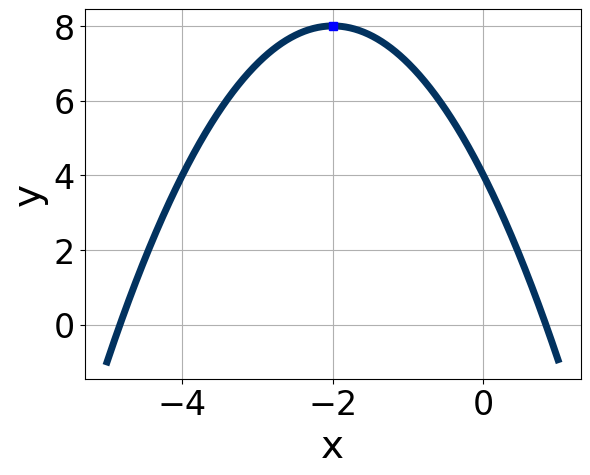
\includegraphics[width=0.5\textwidth]{../Figures/quadraticGraphToEquationCopyB.png}
\end{center}
\begin{enumerate}[label=\Alph*.]
\item \( a \in [0.7, 1.2], \hspace*{5mm} b \in [-5, -1], \text{ and } \hspace*{5mm} c \in [11, 14] \)
\item \( a \in [0.7, 1.2], \hspace*{5mm} b \in [1, 5], \text{ and } \hspace*{5mm} c \in [11, 14] \)
\item \( a \in [-1.6, -0.6], \hspace*{5mm} b \in [1, 5], \text{ and } \hspace*{5mm} c \in [2, 8] \)
\item \( a \in [-1.6, -0.6], \hspace*{5mm} b \in [-5, -1], \text{ and } \hspace*{5mm} c \in [2, 8] \)
\item \( a \in [-1.6, -0.6], \hspace*{5mm} b \in [1, 5], \text{ and } \hspace*{5mm} c \in [-12, -9] \)

\end{enumerate} }
\litem{
Graph the equation below.\[ f(x) = (x-3)^2 - 19 \]\begin{enumerate}[label=\Alph*.]
\begin{multicols}{2}\item 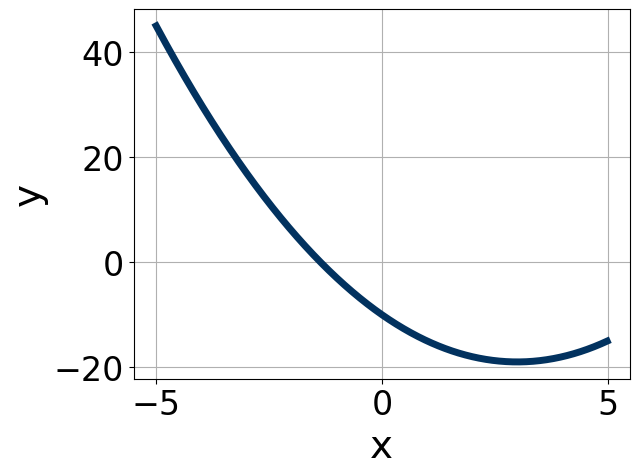
\includegraphics[width = 0.3\textwidth]{../Figures/quadraticEquationToGraphAB.png}\item 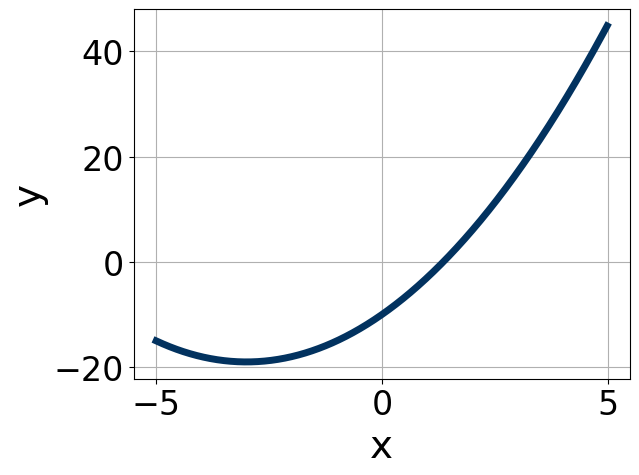
\includegraphics[width = 0.3\textwidth]{../Figures/quadraticEquationToGraphBB.png}\item 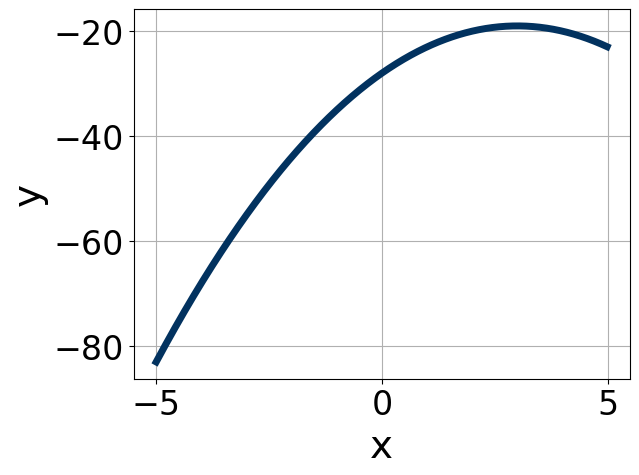
\includegraphics[width = 0.3\textwidth]{../Figures/quadraticEquationToGraphCB.png}\item 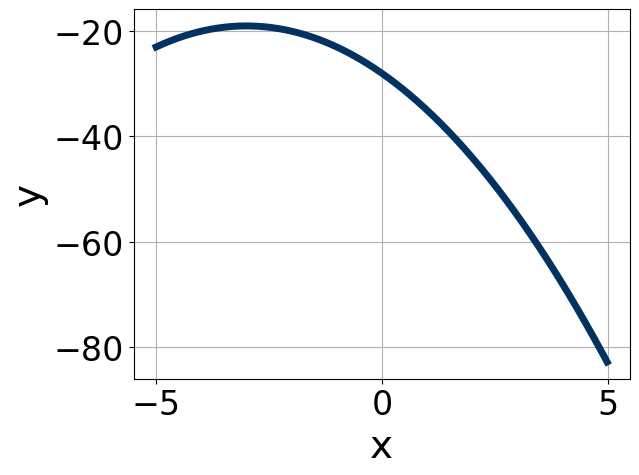
\includegraphics[width = 0.3\textwidth]{../Figures/quadraticEquationToGraphDB.png}\end{multicols}\item None of the above.
\end{enumerate} }
\litem{
Solve the quadratic equation below. Then, choose the intervals that the solutions $x_1$ and $x_2$ belong to, with $x_1 \leq x_2$.\[ 25x^{2} -10 x -24 = 0 \]\begin{enumerate}[label=\Alph*.]
\item \( x_1 \in [-0.53, -0.11] \text{ and } x_2 \in [2.39, 2.69] \)
\item \( x_1 \in [-4.11, -3.68] \text{ and } x_2 \in [0.03, 0.52] \)
\item \( x_1 \in [-1.71, -1.45] \text{ and } x_2 \in [0.31, 0.65] \)
\item \( x_1 \in [-0.87, -0.62] \text{ and } x_2 \in [1.01, 1.56] \)
\item \( x_1 \in [-20.08, -19.94] \text{ and } x_2 \in [29.98, 30.43] \)

\end{enumerate} }
\litem{
Factor the quadratic below. Then, choose the intervals that contain the constants in the form $(ax+b)(cx+d); b \leq d.$\[ 54x^{2} +15 x -25 \]\begin{enumerate}[label=\Alph*.]
\item \( a \in [1.7, 3.3], \hspace*{5mm} b \in [-9, -4], \hspace*{5mm} c \in [17.44, 18.8], \text{ and } \hspace*{5mm} d \in [5, 7] \)
\item \( a \in [-0.7, 2.4], \hspace*{5mm} b \in [-30, -22], \hspace*{5mm} c \in [0.21, 1.23], \text{ and } \hspace*{5mm} d \in [44, 48] \)
\item \( a \in [23.7, 27.8], \hspace*{5mm} b \in [-9, -4], \hspace*{5mm} c \in [1.83, 3.14], \text{ and } \hspace*{5mm} d \in [5, 7] \)
\item \( a \in [8.3, 10.3], \hspace*{5mm} b \in [-9, -4], \hspace*{5mm} c \in [5.77, 7.09], \text{ and } \hspace*{5mm} d \in [5, 7] \)
\item \( \text{None of the above.} \)

\end{enumerate} }
\litem{
Graph the equation below.\[ f(x) = -(x+4)^2 - 18 \]\begin{enumerate}[label=\Alph*.]
\begin{multicols}{2}\item 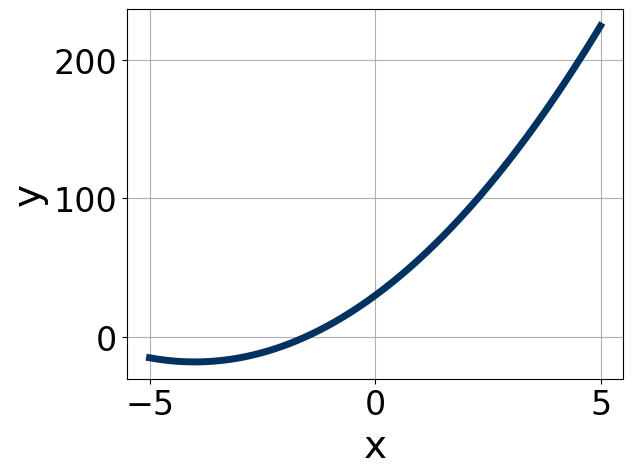
\includegraphics[width = 0.3\textwidth]{../Figures/quadraticEquationToGraphCopyAB.png}\item 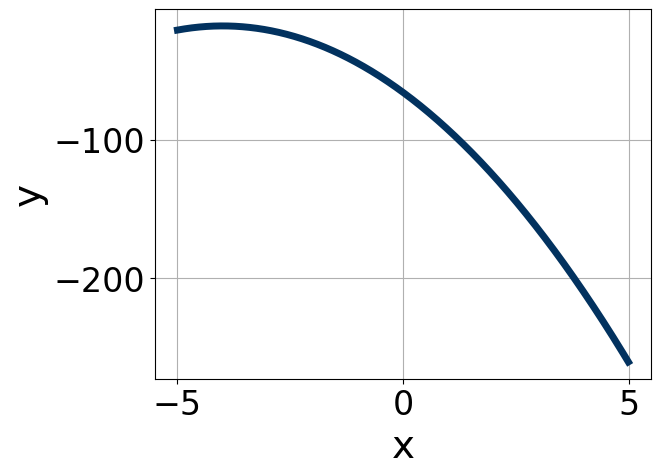
\includegraphics[width = 0.3\textwidth]{../Figures/quadraticEquationToGraphCopyBB.png}\item 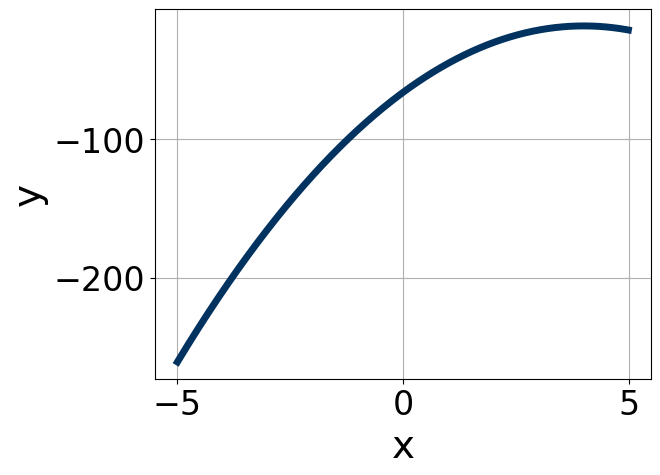
\includegraphics[width = 0.3\textwidth]{../Figures/quadraticEquationToGraphCopyCB.png}\item 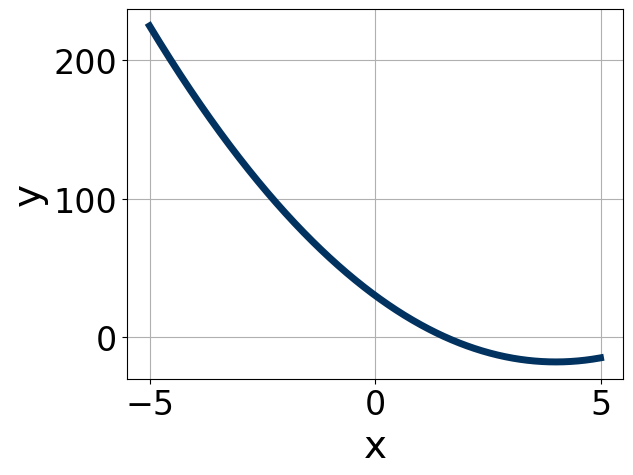
\includegraphics[width = 0.3\textwidth]{../Figures/quadraticEquationToGraphCopyDB.png}\end{multicols}\item None of the above.
\end{enumerate} }
\litem{
Solve the quadratic equation below. Then, choose the intervals that the solutions belong to, with $x_1 \leq x_2$ (if they exist).\[ 19x^{2} -13 x -5 = 0 \]\begin{enumerate}[label=\Alph*.]
\item \( x_1 \in [-6.3, -3.2] \text{ and } x_2 \in [17.66, 18.29] \)
\item \( x_1 \in [-23.7, -22.4] \text{ and } x_2 \in [23.22, 24.85] \)
\item \( x_1 \in [-1.7, -0.7] \text{ and } x_2 \in [0.21, 0.88] \)
\item \( x_1 \in [-0.5, 0.3] \text{ and } x_2 \in [0.8, 1.6] \)
\item \( \text{There are no Real solutions.} \)

\end{enumerate} }
\litem{
Write the equation of the graph presented below in the form $f(x)=ax^2+bx+c$, assuming  $a=1$ or $a=-1$. Then, choose the intervals that $a, b,$ and $c$ belong to.
\begin{center}
    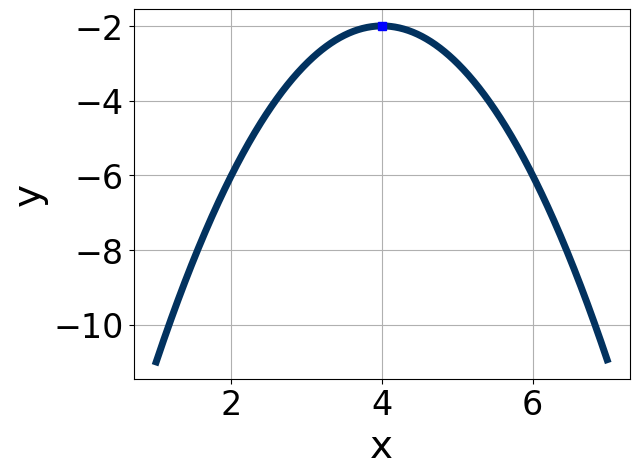
\includegraphics[width=0.5\textwidth]{../Figures/quadraticGraphToEquationB.png}
\end{center}
\begin{enumerate}[label=\Alph*.]
\item \( a \in [-1, 0], \hspace*{5mm} b \in [-8, -4], \text{ and } \hspace*{5mm} c \in [-18, -16] \)
\item \( a \in [0, 4], \hspace*{5mm} b \in [-8, -4], \text{ and } \hspace*{5mm} c \in [14, 16] \)
\item \( a \in [-1, 0], \hspace*{5mm} b \in [-8, -4], \text{ and } \hspace*{5mm} c \in [-16, -10] \)
\item \( a \in [0, 4], \hspace*{5mm} b \in [6, 9], \text{ and } \hspace*{5mm} c \in [14, 16] \)
\item \( a \in [-1, 0], \hspace*{5mm} b \in [6, 9], \text{ and } \hspace*{5mm} c \in [-18, -16] \)

\end{enumerate} }
\end{enumerate}

\end{document}